\section{Estratégia de Busca}\label{sec:est_busca}
A estratégia de busca utilizada para gerar os novos
estados a partir do estado atual $x$ é apresentada na
figura~\ref{fig:estr_busca}.

\begin{figure}[H]
  \centering
  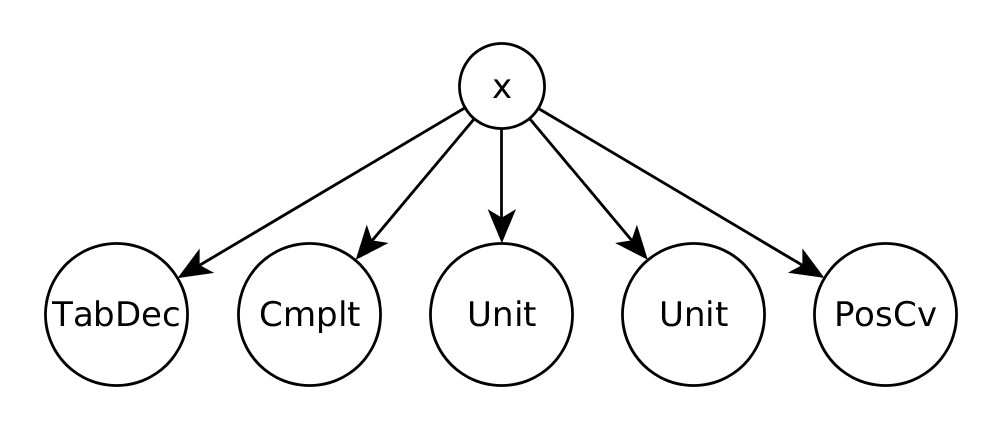
\includegraphics[width= 0.8\linewidth]{tab_dec}
  \caption{Ilustração da distribuiçao dos tabuleiros
           considerados no planejamento}\label{fig:estr_busca}
\end{figure}

Os tipos de ações que são geradas são:
\begin{itemize}
  \item \textit{TabDec}: Ação escolhida no último planejamento
  \item \textit{Unit}: Ação gerada a partir da tabela de decisão
        onde a ação de um único robô foi modificada
  \item \textit{Cmplt}: Ação gerada a partir da tabela de decisão
        onde a ação do time completo foi modificada
  \item \textit{PosCv}: Ação gerada utilizando posições chave
        (vide secção~\ref{subsec:pos_chave})
\end{itemize}

\subsection{Distribuição da Ação $Mover(r)$}\label{subsec:distr_mov}

Para gerar as ações do tipo $Mover(r)$, são utilizadas três distribuições
uniformes circulares, conforme apresentado na Figura~\ref{fig:distr_mov}. Esta
distribuição é centrada em cada robô.

\begin{figure}[H]
  \centering
  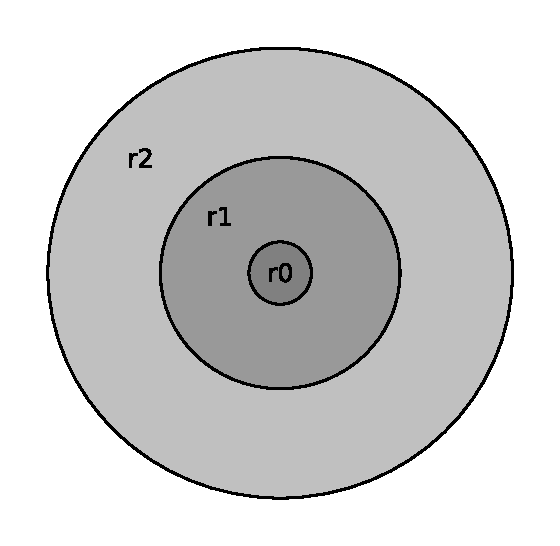
\includegraphics[width=0.5\linewidth] {distr_mov}
  \caption{Distribuição da Ação $Mover(r)$}\label{fig:distr_mov}
\end{figure}

% vim: tw=80 et ts=2 sw=2 sts=2 ft=tex

\subsection{Tabela de Decisão}\label{sec:tab_dec}

A tabela de decisão contém a memória das últimas decisões $a_{anterior} \in A_c$
de todos os robôs de $T_c$.  Isso é incorporado na próxima rodada do algorítimo,
conforme ilustrado na Figura~\ref{fig:estr_busca}.


Devido a movimentação dos robôs em $Rob_{ad}$, somente as ações $Mover(r_i)$ e
$Chutar(r_{com{\ }bola})$ são guardadas integralmente. No caso da ação
$Passar(r_j, r_{com{\ }bola})$, devido a restrição de o robô que recebe
interceptar a bola antes dos robôs em $Rob_{ad}$, o cálculo do receptor $r_j$ é
feito a cada rodada. O receptor anterior só entra no custo da mudança (vide
Seção~\ref{subsec:change_cost}).

Caso a posse de pola passe para o time adversário, o robô que possuía a bola
anteriormente fica com a sua última ação do tipo $Mover(r_i)$.

% vim: tw=80 et ts=2 sw=2 sts=2 ft=tex

\subsection{Posições Chave}\label{subsec:pos_chave}

Devido ao grande número de possibilidades para as posições dos robôs, somente a
geração de posições aleatórias não gera bons resultados para as ações do tipo
$Mover(r_i)$. Portanto, para direcionar a busca, foi desenvolvida uma maneira de
se sugerir posições para as ações em questão com o auxílio da interface gráfica.
A Figura~\ref{fig:pos_chave_barreira} mostra a sugestão de uma barreira.  Já na
Figura~\ref{fig:pos_chave_lateral} são sugeridas posições laterais.

\begin{figure}[H]
  \centering
  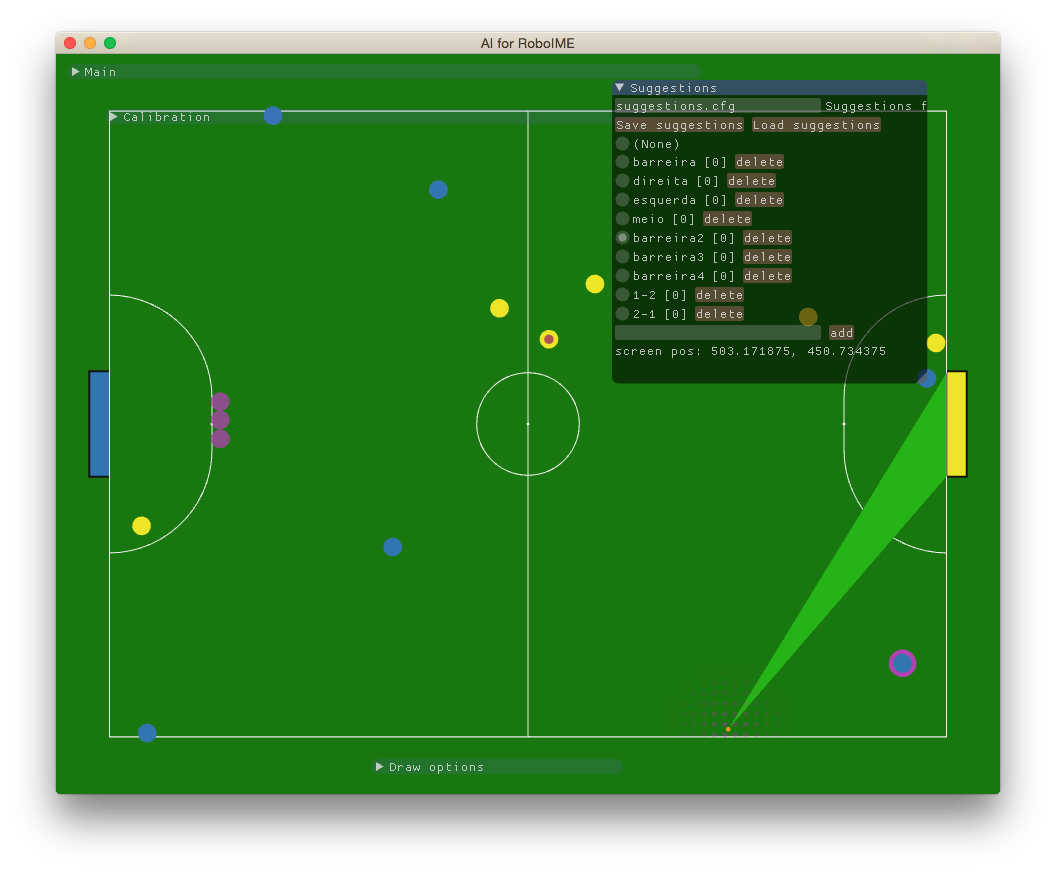
\includegraphics[width= 0.8\linewidth]{pos_chave_barreira}
  \caption{Sugestão de uma barreira (em rosa)}\label{fig:pos_chave_barreira}
  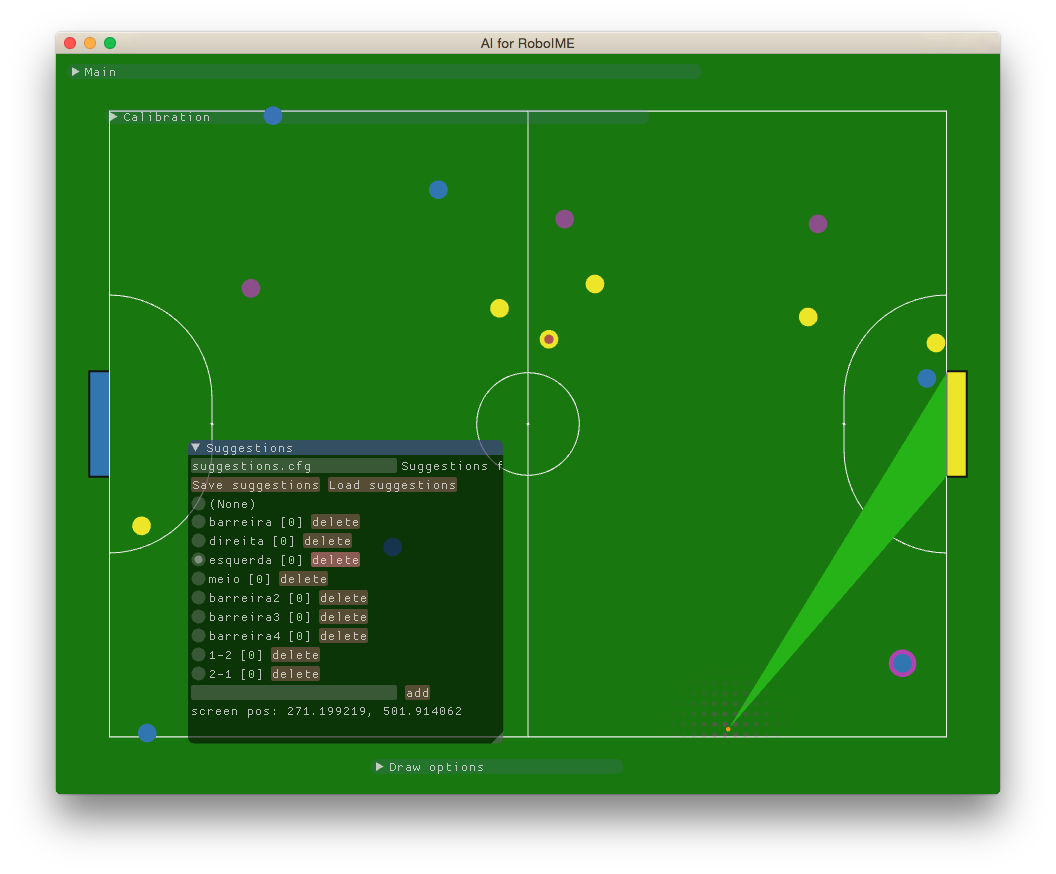
\includegraphics[width= 0.8\linewidth]{pos_chave_lateral}
  \caption{Sugestão de posições laterais (em rosa)}\label{fig:pos_chave_lateral}
\end{figure}

Com o objetivo de verificar a utilidade das posições chave, foi criada uma
maneira de identificar se uma posição chave foi utilizada.

As posições chave são utilizadas das seguinte maneira:
\begin{itemize}
  \item Caso um número de posições inferior ao número de robôs sejam sugeridas,
    são criadas ações aleatórias para completar a sugestão;
  \item As posições sugeridas são atribuídas para o robô mais próximo da posição
    sugerida. Isso é feito na ordem em que as posições foram sugeridas.
\end{itemize}

% vim: tw=80 et ts=2 sw=2 sts=2 ft=tex spelllang=pt_br,en

